\begin{tikzpicture}[node distance=1ex, auto]
\tikzstyle{pict} = [inner sep=0px]
\node[pict] (b) {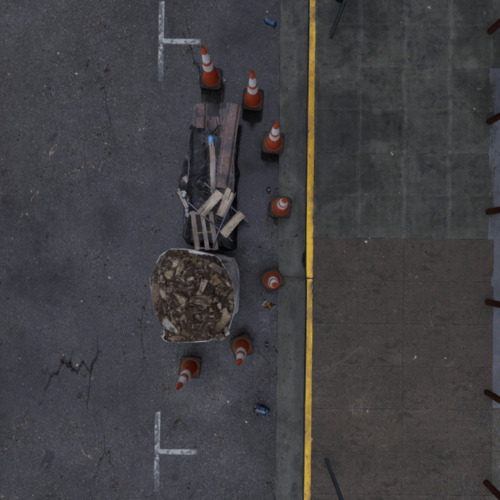
\includegraphics[width=0.25\linewidth]{figs/samples/8.jpg}};
\node[pict, left=of b] (a) {
\includegraphics[width=0.25\linewidth]{figs/samples/6.jpg}};
\node[pict, right=of b] (c) {
\includegraphics[width=0.25\linewidth]{figs/samples/1.jpg}};
\node[pict, below=of a] (d) {
\includegraphics[width=0.25\linewidth]{figs/samples/14.jpg}};
\node[pict, right=of d] (e) {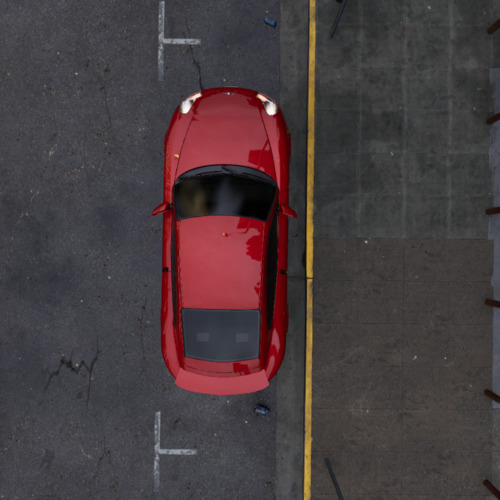
\includegraphics[width=0.25\linewidth]{figs/samples/9.jpg}};
\node[pict, right=of e] (f) {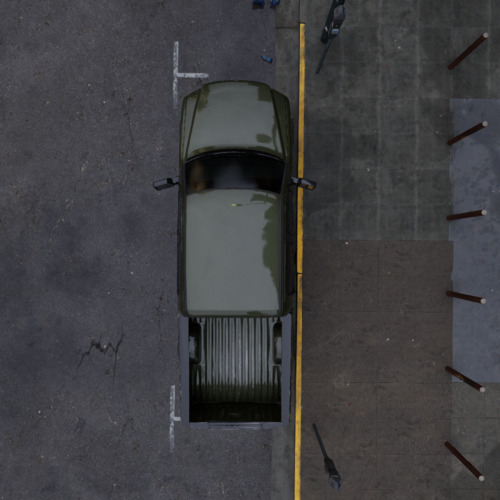
\includegraphics[width=0.25\linewidth]{figs/samples/10.jpg}};

\node[pict, above=of b] {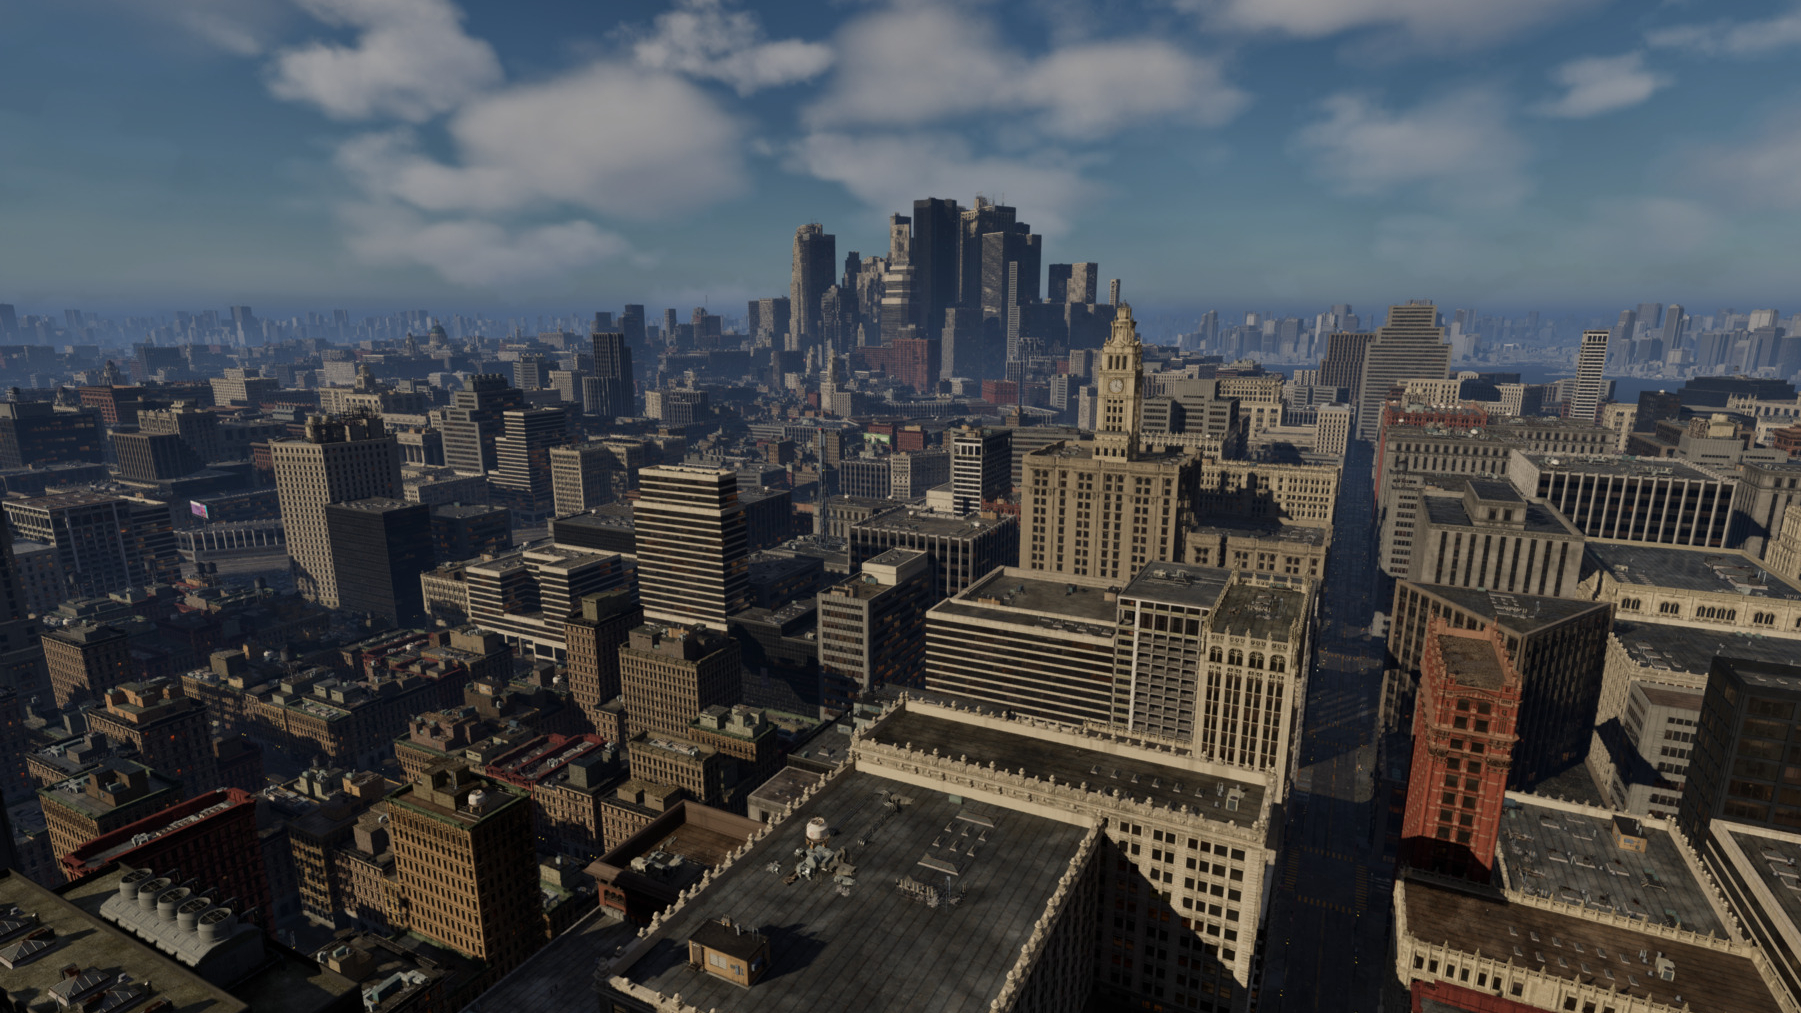
\includegraphics[width=0.8\linewidth]{figs/samples/HighresScreenshot00000.jpg}};
\end{tikzpicture}